%! Author = louis
%! Date = 6/16/20
\documentclass[10pt,a4paper]{article}

\renewcommand{\familydefault}{\sfdefault}
\setlength{\parindent}{0pt}

\usepackage{../Summary}

\hyphenation{
	Kon-text-wech-sel
}

\renewcommand{\lecture}{Betriebssysteme}
\renewcommand{\student}{Louis Seubert}

\usepackage{enumitem}
\setlist[description]{style=nextline,noitemsep}
\setlist{nolistsep,noitemsep}

\usepackage{multicol}
\setlength{\columnseprule}{0.5pt}

\usepackage{color}
\usepackage{standalone}

\usepackage{tikz}
\usetikzlibrary{arrows,automata,petri,trees}

% Document
\begin{document}
\begin{multicols*}{4}
\section{Allgemeines}\label{sec:allgemeines}

\subsection{Aufgaben eines\\Betriebssystems}\label{subsec:aufgaben-eines-betriebssystems}
\begin{itemize}
	\item Betriebsmittelverwaltung
	\item Abstraktions Schnittstellen bereitstellen
\end{itemize}

\subsection{Arten von Betriebsmitteln}\label{subsec:arten-von-betriebsmitteln}

\begin{description}
	\item[Aktive Betriebsmittel]
	      Prozessoren, I/O Controller
	\item[Passives Betriebsmittel, exklusiv]
	      Drucker
	\item[Passives Betriebsmittel, räumlich aufteilbar]
	      Hauptspeicher, Festplatten
	\item[Logische und abstrakte Betriebsmittel]
	      Entstehen aus physikalischen aktiven oder passiven Betriebsmitteln,
	      welche durch eine Software Schicht überlagert werden (Netzwerkverbindungen)
\end{description}

\subsubsection{Ziele der Betriebsmittelverwaltung}
\begin{itemize}
	\item Komfortable Programmierschnittstellen
	\item Abstraktion von den physischen Geräten und Unabhängigkeit
	\item Abstraktion der Hardware durch Software Schnittstellen (Dateisysteme, statt festplatten)
	\item Effizienzsteigerung durch Optimierungen von Abläufen
\end{itemize}

\subsection{Hardware \& Betriebssystem}\label{subsec:hardware-betriebssystem}
Hardware und Software sind logisch äquivalent.
Hardware ist nur versteinerte Software.

\section{Prozessverwaltung}\label{sec:prozessverwaltung}

\subsection{Prozesse}

\textbf{Grundlegendes Konzept}\hfill\\
\textcolor{red}{Ein Prozess ist ein in Ausführung befindliches Programm}, somit ist
ein Prozess die Abfolge der Ausführungen von Instruktionen dieses Programmes.

\textbf{Vorgehen bei Ausführung von\\Programmen}\hfill
\begin{enumerate}
	\item Erzeugen eines neuen Prozesses pro Ausführung eines Programmes durch das Betriebsystem
	\item Anlegen eines neuen Eintrag in der \textbf{Prozesstabelle}
\end{enumerate}

\subsubsection{Prozesstabelle}\label{subsubsec:prozesstabelle}

Die \textbf{Prozesstabelle} verwaltet alle dem Betriebsystem bekannten Prozesse mit \textbf{Process Control Blocks},
in diesen Blöcken befinden sich Informationen:
\begin{itemize}
	\item CPU Registerwerte (SP,PC)
	\item Speicherbelegungen
	\item Berechtigungen
	\item Datei-Handle
\end{itemize}

\subsubsection{Prozesszustände}\label{subsubsec:prozesszustände}

Alle Prozesse werden von dem Betriebsystem in einer Datenstruktur gespeichert. Bei dieser Speicherung wird eine
Trennung der Prozesse anhand der Zuständen vorgenommen. Ein \textbf{jeder Prozess} ist seine \textbf{eigene Einheit}
und besitzt somit einen eigenen Befehlszähler und einen internen Zustand:

\begin{center}
	\includestandalone[width=.65\linewidth]{assets/01-figure}
\end{center}

\subsubsection{Prozesszustände Erweiterung}\label{subsubsec:prozesszustände-erweiterung}

Die bisher bekannten Zustände für einen Prozess könne auch erweitert werden:

\textbf{Zustand Blockiert}\hfill
\begin{itemize}
	\item Prozess geht selbstständig in diesen Zustand, nie durch anderen Prozess
	\item Unterscheidung in
	      \begin{itemize}
		      \item Warten auf Taktgeber
		      \item Warten auf ein/ausgabe
		      \item Warten auf ein/ausgabe Gerät
	      \end{itemize}
\end{itemize}

\textbf{Zustand Suspendiert}\hfill
\begin{itemize}
	\item Laden ohne Starten
	\item Prozess kann nur mit Hilfe eines Übergeordneten Prozesses/Systemaufrufes wieder gestartet werden
\end{itemize}

\textbf{ Zustand Blockiert/Suspendiert}\hfill
\begin{itemize}
	\item Kombination Blockiert/Suspendiert
	\item Nach Ereigniseintritt nur noch Suspendiert
	\item Nach Freigabe nur noch Blockiert
\end{itemize}

\textbf{ Zustand nicht-existent}\hfill
\begin{itemize}
	\item dem Betriebssystem nicht mehr bekannt
	\item nach Beendigung oder vor Laden
\end{itemize}

\subsubsection{Prozesswechsel}\label{subsubsec:prozesswechsel}
Der Prozesswechsel sieht vor das der CPU abwechselnd unterschiedliche Prozesse zugeteilt werden, welche als
nächstes ausgeführt werden. Bei einem Übergang von einen auf den anderen Prozess werden die aktuellsten
Informationen wie der \emph{Kontext der CPU Register} und der \emph{Memory Management Unit} in den PCB geschrieben
und somit gespeichert.

\textbf{Prozess Auswahl}\hfill\\
Mit Hilfe von \emph{Prioritäten} wird ein Prozess aus der Bereitliste ausgewählt. Diese Prioritäten sind abbildbar
auf die restfristen für die Prozess-Antworten.

\textbf{Prozess-Verdrängung}\hfill\\
Sollte ein Prozess zu ende sein oder er blockiert sich selbst, so gibt es \emph{automatisch} den Prozessor frei.
Sollte er nicht eigenständig den Prozessor freigen so wird nach Ablauf seiner Rechenzeit vom Betriebsystem
verdrängt. Dabei werden die \textbf{PCB} und die \textbf{TCB} gesichert.

\subsection{Threads}\label{subsec:threads}

Ein \textbf{Prozess} enthält \textit{einen oder mehrere} \textbf{Threads}. Threads teilen sich gewisse
Speicherbereiche und Adressräume. Bei einem \textbf{Zugriff} auf gemeinsame Daten sind
\textbf{Synchronisationsmechanismen} erforderlich, um \textbf{Laufzeitabhängigkeiten} (race conditions) zu vermeiden.
Jeder Thread besitzt ebenso \textbf{eigene} Register und einen eigenen Stack, ähnlich wie Prozesse.

Ähnlich wie es bei einem Prozess den Process Control Block gibt, so gibt es bei einem Thread den
\textbf{Thread Control Block} (TCB), dieser ist ähnlich wie der PCB und speichert ebenso Informationen. Zudem wird
aber noch eine \textbf{referenz auf den PCB} des dazugehörigen Prozesses gespeichert.

\subsubsection{User- und Kernel-Level-Threads}\label{subsubsec:user-kernel-level-threads}

\textbf{User-Level-Thread}\hfill\\
Ist durch den Softwareentwickler \textit{explizit} erstellt
worden um eine parallelisierung zu ermöglichen.

\textbf{Kernel-Level-Thread}\hfill\\
Sind die tatsächlich auf der CPU laufenden Prozesse welche
dem Betriebssystem bekannt sind, und von diesen verwaltet werden.

\textbf{Zuordnung zwischen ULT und KLT}\hfill
\begin{itemize}
	\item \textbf{m:1} das Multithreading findet in der Laufzeitumgebung statt
	\item \textbf{1:1} das Multithreading findet auf der Ebene des Betriebsystems statt
	\item \textbf{n:m} Hybridlösung
\end{itemize}

\subsubsection{Multithreading}\label{subsubsec:multithreading}
Vervielfachung der Steuerlogik um schnelle Prozesswechsel zu ermöglichen. Jeder dieser so gewonnen Hardware Threads
wird wie logischer Prozessor Core vom Betriebssystem angesehen.

\subsection{Speicherbelegung}\label{subsec:speicherbelegung}
Prozesse und Threads arbeiten auf einem Virtuellen Adressraum. Die Speicherverwaltung des Betriebssystems
konvertiert die virtuellen Adressen in physische Adressen. Dort werden die Prozesse dann ausgeführt.

\subsection{Prozess Scheduling}\label{subsec:prozess-scheduling}

Der \textbf{Prozess-Scheduler} ist ein Teil des Betriebsystems und bestimmt \textbf{welcher} Prozess für
\textbf{wie lange} die CPU zugeteilt bekommt. Zu dessen Aufgaben gehört auch:
\begin{itemize}
	\item Unterbrechungsbehandlung
	\item Starten und Stoppen von Prozessen
	\item Zuteilung der Prozesse auf die Prozessoren der Hardware
\end{itemize}

\subsubsection{Metriken der Ablaufplanung}\label{subsubsec:metriken-ablaufplanung}
\begin{itemize}
	\item \(t\) benötige Ausführungszeit (Rechenzeit)
	\item \(T\) gesamte Antwortzeit inkl. Wartezeit
	\item \(M := T -t\) Wartezeit auf der Bereitliste
	\item \(R := t / T\) Antwortrate
	\item \(P := T / t\) Verzögerungsrate
\end{itemize}

\subsection{Scheduling Algorithmen}
\subsubsection*{FCFS - First Come First Serve}
\begin{itemize}
	\item Nicht verdrängend, das bedeutet dass der neue Prozesse an das Ende der zu bearbeitenden
	      Bereitliste eingefügt wird und der aktuelle Prozess fertig rechnen kann
	\item Als nächstes bearbeitet wird immer der Prozess welcher am Anfang der Bereitliste steht
	\item Priortäten spielen keine Rolle
\end{itemize}
\textbf{\small Vorteile:}\hfill
\begin{itemize}
	\item Jeder Prozess kommt zum rechnen, keiner kann Aushungern
\end{itemize}
\textbf{\small Nachteile:}\hfill
\begin{itemize}
	\item Prozesse mit vielen Ein- und Ausgaben können stark ausgebremst werden
\end{itemize}
\subsubsection*{SPN - Shortest Process Next}
\begin{itemize}
	\item Die voraussichtliche Rechenzeit aktueller Prozesse muss bekannt sein
	\item Nicht verdrängend, das bedeutet dass der aktueller Prozess fertig rechnen kann und
	      dann der nächste kürzeste Prozess starten kann
	\item Ist optimal hinsichtlich des durchsatzes, wenn alle Prozesse direkt verfügbar sind
\end{itemize}
\subsubsection*{RR - Round Robin}
\begin{itemize}
	\item Nach den Ablauf der Zeitscheibe kommt der aktuell rechnende Prozess an das Ende der Bereitliste
	\item Als nächstes bearbeitet wird immer der Prozess welcher am Anfang der Bereitliste steht
	\item Verdrängend, das bedeutet das neu eintreffende Prozesse an das Ende der Bereitliste kommen
	\item Die Wahl des \textbf{Quantums} (größe der Zeitscheibe) bestimmt die Qualität des Verfahrens
\end{itemize}
\textbf{\small Vorteile:}\hfill
\begin{itemize}
	\item Günstige Antwortzeiten für Prozesse mit kurzen Laufzeiten
\end{itemize}
\textbf{\small Nachteile:}\hfill
\begin{itemize}
	\item Prozesse mit lange Laufzeiten sind benachteiligt
\end{itemize}
\subsubsection*{PSPN - Preemptive Shortest Process Next}
\begin{itemize}
	\item Verdrängend, das bedeutet dass wenn ein Prozess bereit wird, der geringere Restrechenzeit hat dann wird
	      dieser ausgeführt
\end{itemize}
\textbf{\small Vorteile:}\hfill
\begin{itemize}
	\item Neue Prozesse mit kurzer Rechenzeit sind bevorzugt
	\item Die im schnitt beste \textbf{Verzögerungsrate}
\end{itemize}
\textbf{\small Nachteile:}\hfill
\begin{itemize}
	\item Eine neigung zum Aushungern sehr langer Prozesse
\end{itemize}
\subsubsection*{HPRN - Highest Penalty Ratio Next}
\begin{itemize}
	\item Es gibt eine Pseudo Priorität die sich aus der bisherigen Wartezeit und der bisherigen Rechenzeit
	      zusammensetzt
	      \(\text{Penalty} = \cfrac{\text{\small bisherige Wartezeit} + \text{\small bisherigen Rechenzeit}}{\text{\small bisherigen Rechenzeit}}\)
	\item Der Prozess mit der \textbf{größten} Pseudo Priorität bekommt den Prozessor zugeteilt
	\item Das Verfahren ist \emph{nicht verdrängend}
\end{itemize}
\textbf{\small Vorteile:}\hfill
\begin{itemize}
	\item Es kann kein Prozess Aushungern solange ein \(P < 1\) existiert
\end{itemize}
\textbf{\small Nachteile:}\hfill
\begin{itemize}
	\item Die Entscheidungsauswahl kostet Rechenzeit
	\item Es gibt eine Benachteiligung von kurzen Prozessen nach langen
\end{itemize}
\subsubsection*{FB - Multi Level Feedback}
\begin{itemize}
	\item Eine Unterteilung der Bereitliste in mehrere Ebenen mit verschiedenen Priorität
\end{itemize}
\textbf{\small Vorteile:}\hfill
\begin{itemize}
	\item Es ist keine Prioritätenberechnung erforderlich
\end{itemize}
\subsubsection{Multicore Scheduling}
Das Scheduling von Kernel Level Threads
\paragraph{Time Sharing} Scheduling von unabhängigen Threads. Dabei geht der erste bereite Thread an den ersten
bereiten Prozessor Kern.
\paragraph{Space Sharing} Scheduling von Threads des selben Prozesses. Dabei werden alle Threads die zu dem gleichen
Prozess gehören gleichzeitig auf den Kernen ausgeführt.
\paragraph{Gang Sharing} Scheduling von Threads einer Gruppe an anhängiger Threads. Dabei werden alle Threads, die
aufgrund ihrer Abhängigkeit gruppiert werden können, auf den Kernen gleichzeitig ausgeführt.
\section{Prozesssynchronisation}
\subsection{Zeitkritische Abläufe}

\subsubsection*{Zeitkritisch:}
Wenn zwei oder mehrere Threads bzw. Prozesse anhängig sind von ihrer relativen Ausführungsgeschwindigkeit.

\subsubsection*{Wettlaufsituation:}
Eine Abhängigkeiten welche von dem relativen Laufzeitverhalten der Threads bzw. der Prozesse abhängig ist.

\subsubsection*{Vermeiden von Wettlaufsituation:}
Können durch den gegenseitigen Ausschluss (\textcolor{blue}{mutual exclusion}, mutex) bei dem Zugriff auf gemeinsam
genutzt Daten oder Betriebsmittel vermieden werden.

\subsubsection{Semaphore}
\textbf{Prinzip:} Zugriff auf gemeinsame Daten oder Betriebsmittel wird ergänzt durch den Zugriff auf eine
definierte gemeinsame Datenstruktur vom Typ Semaphore, welcher die Kontrolle der Betriebsmittel untersteht.

\subsubsection*{Operationen}
\begin{description}
	\item[P-Operation] Atomare, unteilbare Operation die einen Counter dekrementiert. \\
	      Entspricht dem Zustandsübergang von dem Zustand rechnend in den Zustand blockiert.
	\item[V-Operation] Atomare, unteilbare Operation die einen Counter inkrementiert. \\
	      Entspricht dem Zustandsübergang von dem Zustand blockiert in den Zustand bereit.
\end{description}

\subsubsection*{Eigenschaften}
\begin{itemize}
	\item Es gibt keine Prozessunterbrechung beim ausführen einer der P- bzw. V-Operation
	\item Alle zeitkritischen Abschnitte müssen von allen beteiligten Prozessen mit P- bzw. V-Operationen geklammert
	      werden
	\item Die interne Variablen der Semaphore werden durch das Betriebssystem verwaltet, zugriff nur über die
	      P- bzw. V-Operation möglich. Diese werden auch als \textcolor{blue}{System Calls} bezeichnet.
	\item Es gibt zwei unterschiedliche Arten von Semaphoren: \textcolor{blue}{binär}, \textcolor{blue}{zählend}
\end{itemize}
\subsubsection*{Verwendungsmöglichkeit}
\begin{itemize}
	\item Initial Wert = \textbf{1}\\
	      Wechselseitiger Ausschluss (\textcolor{blue}{binär})
	\item Initial Wert = \textbf{n}\\
	      Bis zu \(n\) verschiedene Prozesse dürfen den kritischen Bereich betreten
	\item Initial Wert = \textbf{0}\\
	      Warten auf die Freigabe durch einen anderen Prozess
\end{itemize}
\subsubsection*{Verklemmung}
Eine zyklische Wartesituation zwischen mehreren Prozessen, wobei jeder beteiligte Prozess auf die Freigabe von
Betriebsmitteln wartet, die ein anderer beteiligter Prozess bereits exklusiv belegt hat.
\section{Petri Netze}
Petri Netze sind ein Modell zur Darstellung und Modellierung von Synchronisation und Kommunikation zwischen
nebenläufigen (parallelen) Abläufen. Dabei werden statische sowie dynamische Abhängigkeiten zwischen Prozessen und
Threads genauer dargestellt.\\
Ein Petrinetz besteht aus Stellen, Transitionen und Kanten. Es ist ein Bipartiter Graph. Dabei sind nie zwei Stellen
oder zwei Transitionen über eine Kante miteinander Verbunden.

\begin{description}
	\item[Stelle] Aufenthaltsbereiche bzw. Teilzustände
	\item[Transitionen] Träger der Aktivitäten
	\item[Kanten] Abhängigkeiten zwischen Stellen und Transitionen
\end{description}

\subsubsection*{Eingangsstellen und Ausgangsstellen}
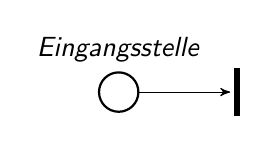
\begin{tikzpicture}[node distance=1.5cm,>=stealth',auto]
	\tikzstyle{place}=[circle, thick, draw=black,minimum size=5mm]
	\tikzstyle{transition hor}=[rectangle, thick, fill=black, minimum width=6mm, inner ysep=1pt]
	\tikzstyle{transition ver}=[rectangle, thick, fill=black, minimum height=6mm, inner xsep=1pt]

	\node [place,tokens=0] (a) [label=above:\textit{Eingangsstelle}]{};
	\node [transition ver] (t1) [right of=a] {}
	edge [pre]                  (a);
\end{tikzpicture}

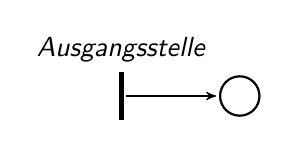
\begin{tikzpicture}[node distance=1.5cm,>=stealth',auto]
	\tikzstyle{place}=[circle, thick, draw=black,minimum size=5mm]
	\tikzstyle{transition hor}=[rectangle, thick, fill=black, minimum width=6mm, inner ysep=1pt]
	\tikzstyle{transition ver}=[rectangle, thick, fill=black, minimum height=6mm, inner xsep=1pt]

	\node [transition ver] (t1) [label=above:\textit{Ausgangsstelle}] {};
	\node [place,tokens=0] (a) [right of=t1] {}
	edge [pre]                 (t1);
\end{tikzpicture}

\subsection{Schaltregeln}
Eine Transition \(t\) kann schalten, wenn alle Stellen \(s\), die eine Kante zu \(t\) besitzen, mindestens eine
Marke besitzen. Wenn eine Transition \(t\) schaltet, wird jeder Stelle \(s\), die eine Kante \textbf{zu} \(t\)
besitzt, eine Marke entnommen, und in jeder Stelle \(s\), die eine Kante \textbf{von} \(t\) besitzt eine Marke
erzeugt.

\subsection{Nebenläufigkeit}
Bei nebenläufigen Transaktionen besteht keine Abhängigkeit zwischen den Transaktionen.

\begingroup
\setlength{\columnseprule}{0pt}
\begin{multicols*}{2}
	\centering
	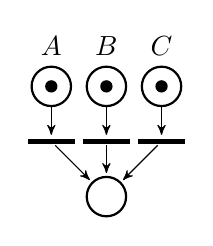
\begin{tikzpicture}[node distance=0.7cm,>=stealth',auto]
		\tikzstyle{place}=[circle, thick, draw=black,minimum size=5mm]
		\tikzstyle{transition hor}=[rectangle, thick, fill=black, minimum width=6mm, inner ysep=1pt]
		\tikzstyle{transition ver}=[rectangle, thick, fill=black, minimum height=6mm, inner xsep=1pt]

		\node [place,tokens=1] (a) [label=above:$A$] {};
		\node [place,tokens=1] (b) [right of=a, label=above:$B$] {};
		\node [place,tokens=1] (c) [right of=b, label=above:$C$] {};
		\node [transition hor] (t1) [below of=a] {}
		edge [pre]             (a);
		\node [transition hor] (t2) [below of=b] {}
		edge [pre]             (b);
		\node [transition hor] (t3) [below of=c] {}
		edge [pre]             (c);
		\node [place,tokens=0] (d) [below of=t2] {}
		edge [pre]             (t1)
		edge [pre]             (t2)
		edge [pre]             (t3);
	\end{tikzpicture}
	\vfill\null\columnbreak
	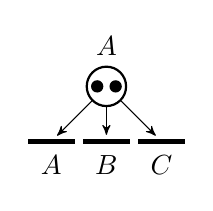
\begin{tikzpicture}[node distance=0.7cm,>=stealth',auto]
		\tikzstyle{place}=[circle, thick, draw=black,minimum size=5mm]
		\tikzstyle{transition hor}=[rectangle, thick, fill=black, minimum width=6mm, inner ysep=1pt]
		\tikzstyle{transition ver}=[rectangle, thick, fill=black, minimum height=6mm, inner xsep=1pt]

		\node [place,tokens=2] (a) [label=above:$A$] {};
		\node [transition hor] (t1) [below of=a, label=below:$B$] {}
		edge [pre]             (a);
		\node [transition hor] (t2) [right of=t1, label=below:$C$] {}
		edge [pre]             (a);
		\node [transition hor] (t3) [left of=t1, label=below:$A$] {}
		edge [pre]             (a);
	\end{tikzpicture}
\end{multicols*}
\endgroup

\subsection{Kausalität und Konflikt}
\begingroup
\setlength{\columnseprule}{0pt}
\begin{multicols*}{2}
	\centering
	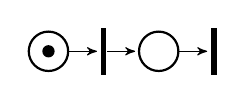
\begin{tikzpicture}[node distance=0.7cm,>=stealth',auto]
		\tikzstyle{place}=[circle, thick, draw=black,minimum size=5mm]
		\tikzstyle{transition hor}=[rectangle, thick, fill=black, minimum width=6mm, inner ysep=1pt]
		\tikzstyle{transition ver}=[rectangle, thick, fill=black, minimum height=6mm, inner xsep=1pt]

		\node [place,tokens=1] (a) [] {};
		\node [transition ver] (t1) [right of=a] {}
		edge [pre]             (a);
		\node [place,tokens=0] (b) [right of=t1] {}
		edge [pre]             (t1);
		\node [transition ver] (t2) [right of=b] {}
		edge [pre]             (b);
	\end{tikzpicture}
	\vfill\null\columnbreak
	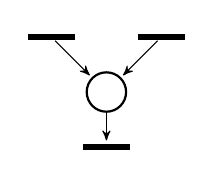
\begin{tikzpicture}[node distance=0.7cm,>=stealth',auto]
		\tikzstyle{place}=[circle, thick, draw=black,minimum size=5mm]
		\tikzstyle{transition hor}=[rectangle, thick, fill=black, minimum width=6mm, inner ysep=1pt]
		\tikzstyle{transition ver}=[rectangle, thick, fill=black, minimum height=6mm, inner xsep=1pt]

		\node [transition hor] (t1) [] {};
		\node [] (blank) [right of=t1] {};
		\node [transition hor] (t2) [right of=blank] {};
		\node [place,tokens=0] (a) [below of=blank] {}
		edge [pre]             (t1)
		edge [pre]             (t2);
		\node [transition hor] (t3) [below of=a] {}
		edge [pre]             (a);
	\end{tikzpicture}
\end{multicols*}
\endgroup

\subsection{Synchronisation}
\begingroup
\setlength{\columnseprule}{0pt}
\begin{multicols*}{2}
	\centering
	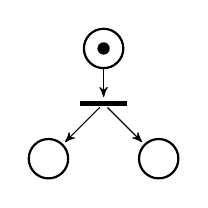
\begin{tikzpicture}[node distance=0.7cm,>=stealth',auto]
		\tikzstyle{place}=[circle, thick, draw=black,minimum size=5mm]
		\tikzstyle{transition hor}=[rectangle, thick, fill=black, minimum width=6mm, inner ysep=1pt]
		\tikzstyle{transition ver}=[rectangle, thick, fill=black, minimum height=6mm, inner xsep=1pt]

		\node [place,tokens=1] (a) [] {};
		\node [transition hor] (t1) [below of=a] {}
		edge [pre]             (a);
		\node [] (blank) [below of=t1] {};
		\node [place,tokens=0] (b) [right of=blank] {}
		edge [pre]             (t1);
		\node [place,tokens=0] (c) [left of=blank] {}
		edge [pre]             (t1);
	\end{tikzpicture}
	\vfill\null\columnbreak
	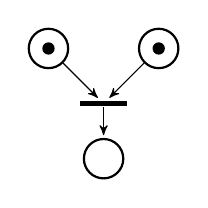
\begin{tikzpicture}[node distance=0.7cm,>=stealth',auto]
		\tikzstyle{place}=[circle, thick, draw=black,minimum size=5mm]
		\tikzstyle{transition hor}=[rectangle, thick, fill=black, minimum width=6mm, inner ysep=1pt]
		\tikzstyle{transition ver}=[rectangle, thick, fill=black, minimum height=6mm, inner xsep=1pt]

		\node [place,tokens=1] (a) [] {};
		\node [] (blank) [right of=a] {};
		\node [place,tokens=1] (b) [right of=blank] {};
		\node [transition hor] (t1) [below of=blank] {}
		edge [pre]             (a)
		edge [pre]             (b);
		\node [place,tokens=0] (c) [below of=t1] {}
		edge [pre]         (t1);
	\end{tikzpicture}
\end{multicols*}
\endgroup

\subsection{Lebendigkeit}
Ein Petrinetz heißt verklemmungsfrei wenn in jeder Markierung eine Transition aktiviert ist, d.h. zu jeder Markierung
gibt es eine nachfolge Markierung.
\begingroup
\setlength{\columnseprule}{0pt}
\begin{multicols*}{2}
	\centering
	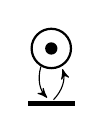
\begin{tikzpicture}[node distance=0.7cm,>=stealth',auto]
		\tikzstyle{place}=[circle, thick, draw=black,minimum size=5mm]
		\tikzstyle{transition hor}=[rectangle, thick, fill=black, minimum width=6mm, inner ysep=1pt]
		\tikzstyle{transition ver}=[rectangle, thick, fill=black, minimum height=6mm, inner xsep=1pt]

		\node [place,tokens=1] (a) [] {};
		\node [transition hor] (t1) [below of=a] {}
		edge [post,bend right] (a)
		edge [pre,bend left]   (a);
	\end{tikzpicture}
	\vfill\par\vspace{1ex}
	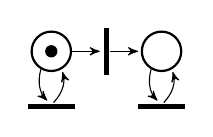
\begin{tikzpicture}[node distance=0.7cm,>=stealth',auto]
		\tikzstyle{place}=[circle, thick, draw=black,minimum size=5mm]
		\tikzstyle{transition hor}=[rectangle, thick, fill=black, minimum width=6mm, inner ysep=1pt]
		\tikzstyle{transition ver}=[rectangle, thick, fill=black, minimum height=6mm, inner xsep=1pt]

		\node [place,tokens=1] (a) [] {};
		\node [transition ver] (t2) [right of=a] {}
		edge [pre]             (a);
		\node [place,tokens=0] (c) [right of=t2] {}
		edge [pre]             (t2);
		\node [transition hor] (t1) [below of=a] {}
		edge [post,bend right] (a)
		edge [pre,bend left]   (a);
		\node [transition hor] (t3) [below of=c] {}
		edge [post,bend right] (c)
		edge [pre,bend left]   (c);
	\end{tikzpicture}
	\vfill\par\vspace{1ex}
	Ein Deadlock freies Petrinetz
	\vfill\par\vspace{1ex}
	\hrule
	\vfill\par\vspace{1ex}
	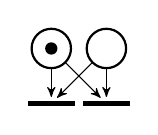
\begin{tikzpicture}[node distance=0.7cm,>=stealth',auto]
		\tikzstyle{place}=[circle, thick, draw=black,minimum size=5mm]
		\tikzstyle{transition hor}=[rectangle, thick, fill=black, minimum width=6mm, inner ysep=1pt]
		\tikzstyle{transition ver}=[rectangle, thick, fill=black, minimum height=6mm, inner xsep=1pt]

		\node [place,tokens=1] (a) [] {};
		\node [place,tokens=0] (b) [right of = a]{};
		\node [transition hor] (t1) [below of=a] {}
		edge [pre]         (b)
		edge [pre]         (a);
		\node [transition hor] (t2) [below of=b] {}
		edge [pre]             (b)
		edge [pre]             (a);
	\end{tikzpicture}
	\vfill\par\vspace{1ex}
	totes Petrinetz
	\vfill\null\columnbreak
	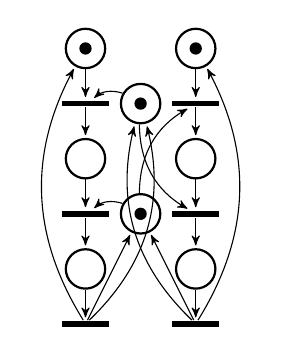
\begin{tikzpicture}[node distance=0.7cm,>=stealth',auto]
		\tikzstyle{place}=[circle, thick, draw=black,minimum size=5mm]
		\tikzstyle{transition hor}=[rectangle, thick, fill=black, minimum width=6mm, inner ysep=1pt]
		\tikzstyle{transition ver}=[rectangle, thick, fill=black, minimum height=6mm, inner xsep=1pt]

		\node [place,tokens=1] (p1) [] {};

		\node [] (blank) [right of=p1] {};

		\node [place,tokens=1] (p2) [right of=blank] {};

		\node [transition hor] (t1) [below of=p1] {}
		edge [pre] (p1);

		\node [place,tokens=1] (p3) [below of=blank] {}
		edge [post, bend right] (t1);

		\node [transition hor] (t2) [below of=p2] {}
		edge [pre] (p2);

		\node [place,tokens=0] (p4) [below of=t1] {}
		edge [pre] (t1);

		\node [place,tokens=0] (p5) [below of=t2] {}
		edge [pre] (t2);

		\node [transition hor] (t3) [below of=p4] {}
		edge [pre] (p4);

		\node [place,tokens=1] (p8) [right of=t3] {}
		edge [post, bend left] (t2)
		edge [post, bend right] (t3);

		\node [transition hor] (t4) [below of=p5] {}
		edge [pre, bend left] (p3)
		edge [pre] (p5);

		\node [place,tokens=0] (p6) [below of=t3] {}
		edge [pre] (t3);

		\node [place,tokens=0] (p7) [below of=t4] {}
		edge [pre] (t4);

		\node [transition hor] (t5) [below of=p6] {}
		edge [pre] (p6)
		edge [post, bend right] (p3)
		edge [post] (p8)
		edge [post,bend left] (p1);

		\node [transition hor] (t5) [below of=p7] {}
		edge [pre] (p7)
		edge [post, bend left] (p3)
		edge [post] (p8)
		edge [post,bend right] (p2);
	\end{tikzpicture}
	\vfill\par\vspace{1ex}
	Ein nicht Deadlock freies Petrinetz
\end{multicols*}
\endgroup

\subsection{Sicherheit}
Ein Petrinetz heißt \textbf{b-sicher}, wenn für jede Markierung die maximale Anzahl an Marken in jeder Stelle höchstens
\(b\) beträgt. Ist \(b = 1\), spricht man von sicher.

\begingroup
\setlength{\columnseprule}{0pt}
\begin{multicols*}{2}
	\centering
	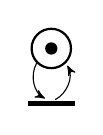
\begin{tikzpicture}[node distance=0.7cm,>=stealth',auto,bend angle=45]
		\tikzstyle{place}=[circle, thick, draw=black,minimum size=5mm]
		\tikzstyle{transition hor}=[rectangle, thick, fill=black, minimum width=6mm, inner ysep=1pt]
		\tikzstyle{transition ver}=[rectangle, thick, fill=black, minimum height=6mm, inner xsep=1pt]

		\node [place,tokens=1] (a) [] {};
		\node [transition hor] (t1) [below of=a] {}
		edge [post,bend right] (a)
		edge [pre,bend left]   (a);
	\end{tikzpicture}
	\hfill\\
	sicheres Petrinetz
	\vfill\null\columnbreak
	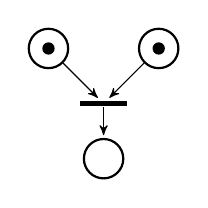
\begin{tikzpicture}[node distance=0.7cm,>=stealth',auto,bend angle=45]
		\tikzstyle{place}=[circle, thick, draw=black,minimum size=5mm]
		\tikzstyle{transition hor}=[rectangle, thick, fill=black, minimum width=6mm, inner ysep=1pt]
		\tikzstyle{transition ver}=[rectangle, thick, fill=black, minimum height=6mm, inner xsep=1pt]

		\node [place,tokens=1] (a) [] {};
		\node [] (blank) [right of=a] {};
		\node [place,tokens=1] (b) [right of=blank] {};
		\node [transition hor] (t1) [below of=blank] {}
		edge [pre]             (a)
		edge [pre]             (b);
		\node [place,tokens=0] (c) [below of=t1] {}
		edge [pre]         (t1);
	\end{tikzpicture}
	\hfill\\
	nicht beschränktes Petrinetz
\end{multicols*}
\endgroup
\subsection{Erweiterungen}
\begin{description}
	\item[Kardinalität] Beschreibt eine Ganzzahlige Anzahl an Marken welche bei einer Schaltung entnommen wird bzw.
	      hinzugefügt wird
	\item[Kapazität] Beschreibt die Anzahl der Marken die eine Stelle aufnehmen kann
	\item[Prioritäten] Transitionen können eine Wahrscheinlichkeit besitzen welche als Priorität aufgefasst wird.
	\item[Farben] Eine Schaltregel ist abhängig von der Farbe der Marke
\end{description}

\section{Speicherverwaltung}

\subsection{Grundlagen}
Die Speicherverwaltung dient der Verwaltung der Laufzeitdaten, dazu zählen vorallem die Verwaltung des freien und
belegeten Speicherplatzes während der Ausführung von Prozessen auf volatilen Speichermedien. Dabei wird vorallem auf
eine effiziente Verwaltung dieser Ressourcen geachtet.

\begin{description}
	\item[Speicherverwaltung] Teil des Betriebssystems, der den flüchtigen Speicher während der Ausführung der Prozesse
	      verwaltet
	\item[Speicherbedarf eines Prozesses] Setzt sich zusammen aus mehreren Komponenten: Vor der Ausführung des Programs
	      ist es der Quellcode bzw. die Data. Während der Ausführung des Programms ist es vorallem der
	      \textbf{Process Control Block} welcher sich zusammen setzt aus Data und dem Stack.
	\item[Speicherverwaltungssysteme] Während der Ausführung von Prozesse können diese zwischen Hauptspeicher und
	      Festplatte verschoben (\textcolor{blue}{Swapping}) werden oder nicht verschoben werden (\textcolor{blue}{Paging}).
\end{description}

\subsection{Monoprogrammierung}
Ein Programmierstiel ohne Auslagerung oder Seitenverwaltung. Es wird immer nur maximal ein Prozess ausgeführt. Der
Hauptspeicher wird zwischen dem Prozess eines Programms und dem Betriebssystem aufgeteilt.

\subsection{Multiprogrammierung}
Speicher wird in \(n\)-Segmente Aufgeteilt, dabei sind diese nicht überlappend und können unterschiedliche Größen haben.
In Abhängigkeit von der Implementierung kann jeder Prozess entweder in eine Warteliste hinter das am best besten
passende Segment angehängt werden. Oder es wird aus einer Liste dem erst best passenstenten Segment zugeordnet.

\subsubsection*{Segment-Tabelle}
Verwaltung des Speicherbereichs, den ein Prozess bei Ausführung im Hauptspeicher benötigt.

\subsubsection{Modellierung}
\begin{itemize}
	\item Ein Prozess Wartet einen Anteil \(p \in\; ]0;1[\) seiner Zeit auf eine Ein- bzw. Ausgabe
	\item Bei \(n\) Prozessen ist die Wahrscheinlichkeit \(p^{n}\) das alle gleichzeitig warten
	\item \textcolor{blue}{\(A = 1 - p^{n}\)} ist somit die CPU Ausnutzung
\end{itemize}

\subsubsection{Relokation und Speicherschutz}
\subsubsection*{Relokationsproblem}
Werden die Programmbefehle beim Laden des Programmes, d.h. beim Starten des Prozesses in den Speicher angepasst
(modifiziert), kann ein feindliches Programm neue Befehle in den Speicher schreiben und zu diesen Springen. Somit
entsteht ein Speicherschutzproblem. Eine Lösung für dieses sind Basis- und Grenzregister.

\subsubsection{Dynamische Speicherbereitstellung}
Laufende Prozesse fordern Speicherbereiche unterschiedlicher Größe an bzw. geben diese frei. Dabei besteht der
\textbf{Stack} aus lokalen Variablen deren Speicherplatz implizit reserviert ist. Und der \textbf{Heap} besteht aus
Variablen welche unabhängig von der der Nutzungszeit sind, diese müssen aber explizit reserviert werden.

\subsection{Verwaltung der verwendeten Speicherbereiche}
\subsubsection*{Bitmaps}
Eine Methode zur verwaltung von dynamisch zugeteilten Speicherbereichen. Dabei repräsentiert eine \(0\) eine freie
Speichereinheit und eine \(1\) eine belegte Einheit. Die Größen der Einheiten ist entwurfsfrage.

\subsubsection*{Liste}
Dabei bezeichnet jeder Listeneintrag einweder einen freien zusammenhängenden Speicherbereich (H) oder einen von einem
Prozess belegten Speicherbereich (P).

\subsection{Zuteilungstrategien}
Es gibt mehrere unterschiedliche herangehensweisen zur Reservierung von Speicher bei Speicheranforderungen von
Prozessen.

\begin{description}
	\item[First Fit] Dabei wird der erste ausreichend großen Speicherbereich belegt
	\item[Next Fit] Ist ähnlich wie FirstFit, jedoch wird die zuletzt gefundene Speicherposition vermerkt und bei der
	      nächsten anfrage ab diese weiter gesucht
	\item[Best Fit] Dabei wird die gesamte Liste durchsucht und der am besten passente Speicherbereich ausgewählt
	\item[Worst Fit] Dabei wird die gesamte Liste durchsucht und der größte verfügbaren Speicherbereich ausgewählt,
	      dadurch werden möglichst große zusammenhängende Bereiche bewahrt
	\item[Quick Fit] Dabei werden getrennte Liste für freie Speicherbereich in gebräuchlichen Größen geführt
\end{description}

\subsection{Buddy Algorithmus}
Ein Verfahren zur Speicherallokierung, zum möglichst passgenauen erfüllen einer Speicheranforderung.

\subsubsection{Binärer Buddy Algorithmus}
\begin{enumerate}
	\item Der gesamte Speicherbereich wird als Speicher der größe \(2^{k}\) angesehen
	\item Bei einer Anforderung wird der Bedarf auf die nächte zweierpotenz \(2^{p}\) aufgerundet und ein entsprechender
	      Bereich gesucht \(p = \lceil\log_{2}(\text{Speicheranforderung})\rceil\)
	\item Sollte es keinen Speicher der größe \(2^{p}\) geben, so wird nach einem doppelt so großen Bereich der größe
	      \(2^{p+1}\) gesucht und dieser in zwei hälften geteilt.
	\item Gibt es auch keinen Speicher der größe \(2^{p+1}\) wird nach einem vier mal so großen Speicher \(2^{p+2}\)
	      gesucht. Dieser wird dann zunächst in \(2 \cdot 2^{p+2}\) zerlegt und dann in \(4 \cdot 2^{p}\)
	\item \textit{\small Schritt 4 kann dabei beliebig oft auftreten}
	\item Sobald Speicher wieder freigegeben wird, wird geprüft, ob zwei Bereiche gleicher größe wieder zusammengefügt
	      werden können
\end{enumerate}

\subsubsection{Fibonacci Buddy Algorithmus}
Die Größen der aktuell freien Speicherbereiche entsprechen den Fibonacci Zahlen als Vielfaches der Basiseinheit.

\begin{minipage}{\linewidth}
	\centering
	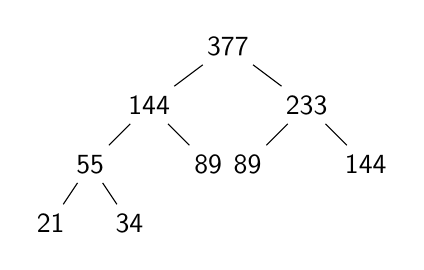
\begin{tikzpicture}[level distance = 0.75cm]
		\tikzstyle{level 1}=[sibling distance = 2cm];
		\tikzstyle{level 2}=[sibling distance = 1.5cm];
		\tikzstyle{level 3}=[sibling distance = 1cm];

		\node {377}
		child {	node {144}
				child{ 	node {55}
						child {	node {21}}
						child {	node {34}}
					}
				child {	node {89}}
			}
		child {	node {233}
				child {	node {89}}
				child {	node {144}}
			};
	\end{tikzpicture}
\end{minipage}

\subsubsection*{Fibonacci Zahlen}
0, 1, 1, 2, 3, 5, 8, 13, 21, 34, 55, 89, 144, 233, 377, 610, 987, 1597, 2584, 4181, 6765, 10946, 17711, 28657, 46368, 75025

\subsubsection{Gewichteter Buddy Algorithmus}
Aufteilung eines Speicherbereichs der Größe \(2^{k+2}\) in zwei Bereiche unterschiedlicher Größe, \(3 \cdot 2^{k}\)
sowie \(2^{k}\). Speicherbereiche der Größe \(3 \cdot 2^{k}\) werden wiederum in zwei Bereiche der Größe \(2^{k+1}\)
sowie \(2^{k}\) gesplittet.

\begin{minipage}{\linewidth}
	\centering
	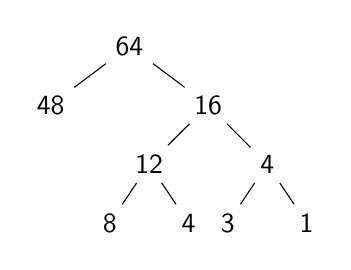
\begin{tikzpicture}[level distance = 0.75cm]
		\tikzstyle{level 1}=[sibling distance = 2cm];
		\tikzstyle{level 2}=[sibling distance = 1.5cm];
		\tikzstyle{level 3}=[sibling distance = 1cm];

		\node {64}
		child {	node {48}}
		child {	node {16}
				child {	node {12}
						child {	node {8}}
						child {	node {4}}
					}
				child {	node {4}
						child {	node {3}}
						child {	node {1}}
					}
			};
	\end{tikzpicture}
\end{minipage}

\subsubsection{Tertiary Buddy Algorithmus}
Aufteilung eines Speicherbereichs der Größe \(2^{k}\) in drei Bereiche unterschiedlicher Größe, \(2^{k-1}\),
\(3 \cdot 2^{k-3}\) sowie \(2^{k-3}\). Speicherbereiche der Größe \(3 \cdot 2^{k-3}\) werden wiederum in zwei Bereiche
der Größe \(2^{k-2}\) sowie \(2^{k-3}\) gesplittet.

\begin{minipage}{\linewidth}
	\centering
	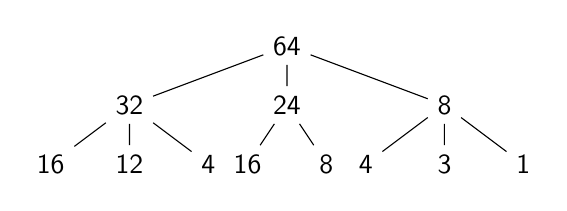
\begin{tikzpicture}[level distance = 0.75cm]
		\tikzstyle{level 1}=[sibling distance = 2cm];
		\tikzstyle{level 2}=[sibling distance = 1cm];

		\node {64}
		child {	node {32}
				child {	node {16}}
				child {	node {12}}
				child {	node {4}}
			}
		child {	node {24}
				child {	node {16}}
				child {	node {8}}
			}
		child {	node {8}
				child {	node {4}}
				child {	node {3}}
				child {	node {1}}
			};
	\end{tikzpicture}
\end{minipage}

\subsection{Swapping}
Bei Timesharing Systemen kann es vorkommen, dass nicht genügend Hauptspeicher für alle rechenbereiten Prozesse vorhanden
ist. Bei Swapping wird jeder Prozess in den Hauptspeicher geladen, dort darf dieser eine gewisse Zeit laufen und wird
anschließend wieder auf die Festplatte ausgelagert. \\
\textbf{Ein- bzw. Auslagerung von Prozessen kann beim Swapping die Speicherzuteilung ändern.} Dabei ändert sich die
Anzahl, Größe und Ort der Bereiche da diese nicht fest stehen sondern dynamisch sind.

\subsubsection*{Problem}
Es stellt sich dabei die Frage wie viel Speicher pro Prozess reserviert werden soll bzw. wann soll der Prozess erzeugt
werden und wann wieder ausgelagert werden.

\subsubsection*{Segmente}
Der Speicherbedarf von Prozessen wird in Segmente untergliedert, diese stellen logische Teile des gesamten
Speicherbereiches dar. Der \textbf{Stack} ist hierbei für lokale Variablen, Methoden etc. und der \textbf{Heap} für
dynamische Variablen bzw. Objekte.

\subsection{Virtueller Speicher}
Sollte der Speicherbedarf zu groß sein für verfügbaren physischen Hauptspeicher, kann das Betriebsystem keine
Anforderung mehr erfüllen. Daher gibt es \textbf{Virtueller Speicher} welcher von dem Betriebsystem verwaltet wird.
Dabei muss der Speicherbedarf eines ausgeführten Programmes nicht unbedingt vollständig im Hauptspeicher untergebracht
sein.

\subsubsection*{Demand Paging}
Lade nur augenblicklich benötigte Speicherbereiche in den Hauptspeicher

\subsubsection*{Lokalität der Referenz}
Prozesse beschränken in der Regel ihre Speicherzugriffe in jeder Phase ihrer Ausführung auf einen relativ kleinen Teil
ihrer zugeordneten Seitenrahmen

\subsubsection*{Arbeitsbereich}
Das \textcolor{blue}{Working Set} ist eine Menge von Seitenrahen welche ein Prozess zu einem bestimmten Zeitpunk
benutzt.

\subsubsection*{Seitenflattern}
Das \textcolor{blue}{Thrashing} kommt dann vor wenn der verfügbare Hautspeicher nicht für alle Seitenrahmen ausreicht
und ein Prozess dennoch auf alle Rahmen zugreift. Dadurch wird das gesamte System sehr langsam da das Betriebsystem nun
ständig Seitenrahmen auf den Sekundär Speicher auslagern muss und einen anderen lesen muss.

\subsubsection*{Virtuelle Adressen}
Speicheradressen im virtuellen Adressraum eines Prozesses

\subsubsection*{Adressketten}
Adressketten setzten sich dabei zusammen aus mehreren Bestandteilen wie:
\begin{itemize}
	\item Namen, welcher für den Menschen lesbar ist
	\item Programmadressen, welche von der CPU benutzt werden
	\item Speicheradressen, welche von der Hardware realisiert ist
\end{itemize}
\[\text{\small Namen}\rightarrow\text{\small Programmadressen}\rightarrow\text{\small Speicheradressen}\]

\subsubsection*{Memory Management Unit - MMU}
Die Memory Management Unit ist verantwortlich für die Umwandlung von Adressen aus dem \textbf{virtuellen Adressraum}
(virtuelle Seiten) in den \textbf{physischen Adressraum} (Seitenrahmen). Dabei haben Seiten und Seitenrahmen haben in
einem Rechnersystem immer die selbe Größe. Zwischen Arbeitsspeicher und Festplatte werden immer komplette Seiten
übertragen.

Dabei gibt es das \textbf{Present bzw. Absent-Bit} welches angibt ob eine virtuelle Seite auf den physischen Speicher
abgebildet wird oder nicht.

Es tritt ein \textbf{Seitenfehler} auf wenn auf ein virtuelle Seite zugegriffen wird welche noch nicht im Hauptspeicher
vorhanden ist und erst geladen werden muss.

\paragraph{Vorgehensweiße}\hfill\\
Beispiel für eine 16 Bit-Adresse mit 4096 Bytes (\(2^{12}\)) Seitengröße
\begin{itemize}
	\item \(16 - 12 = 4\) Eine Zerlegung in 4 Bits für die Seitennummer und 12 Bits Offset
	\item \(2^{4} = 16\) Seiten adressierbar
	\item \(2^{12} = 4096\) Bytes pro Seite adressierbar
	\item \textbf{Seitenummer dient als Index für die Seitentabelle}
	\item Die 12 Bit Offset werden unverändert übernommen und mit \(n\) Bits des Seitenrahmens zur physischen \(12 + n\)
	      Bit Adresse (ohne Present bzw. Absent Bit)
\end{itemize}

\paragraph{Beispiel}\hfill\\
Die Phisische Adresse umfasst \(35\;\texttt{Bit}\). Die Seitengröße beträgt \(2^{13}\;\texttt{Byte}\). Es stehen
\(2^{35}\;\text{Seiten}\) zur Verfügung. Jeder Eintrag in der Seitentabelle belegt 128 \texttt{Bit}.

\begin{enumerate}
	\item\textbf{Größe des Hauptspeichers}\hfill\\
	      Seitengröße entspricht der Größe des Seitenrahmens: \(2^{13}\). \\
	      Somit 13 \texttt{Bit} für die Adressierung in einer Seite. \\
	      \(35 - 13 = 22\;\texttt{Bit}\) für Adressierung des Seitenrahmens in der Physischen Adresse. \\
	      \(2^{22}\;\text{Seitenrahmen} \cdot 2^{13}\;\texttt{Byte} = 2^{35}\;\texttt{Byte}\) Hauptspeicher.
	\item\textbf{Größe des Virtuellen Adressraums}\hfill\\
	      Virtuelle Adressraum umfasst \(2^{35}\;\text{Seiten}\) \\
	      \(35\;\texttt{Bit}\) für Adressierung der Seite. \\
	      \(35 + 13 = 48\;\texttt{Bit}\) für Virtuelle Adresse. \\
	      \(2^{48}\;\texttt{Byte}\) Virtueller Adressraum
	\item\textbf{Speicherbedarf}\hfill\\
	      Eine Seite umfasst \(2^{13}\;\texttt{Byte}\) \\
	      Maximal \(2^{9}\;\text{Prozesse}\) mit jeweils \(2^{48}\;\texttt{Byte}\) Adressraum \\
	      \(2^{9} \cdot 2^{48} = 2^{57}\;\texttt{Byte}\) für alle Prozesse \\
	      \(2^{57} \div 2^{13}\;\texttt{Byte} = 2^{44}\;\text{Seiten}\)
	\item\textbf{Seiten für Seitentabellen}\hfill\\
	      \(2^{9}\;\text{Prozesse}\;\cdot 2^{35}\;\text{Seiten}\;\cdot 2^{4}\;\texttt{Byte}\) \\
	      \(2^{48} \div 2^{13} = 2^{35}\;\text{Seiten für Seitentabellen}\)
\end{enumerate}

\paragraph{Beispiel}\hfill\\
Der Speicherbedarf eines Prozesses in in vier gleich große Segmente unterteilt und für jedes Segment ist ein
Seitentabelle mit maximal acht Einträgen vorgesehen. Die größe einer Seite beträgt \(2^{11}\;\texttt{Byte}\).

\begin{enumerate}
	\item\textbf{Maximale Segmentgröße}\hfill\\
	      \(8\;\text{Seiten} \cdot 2^{11}\;\texttt{Byte}\text{pro Seite} = 2^{14}\;\texttt{Byte}\)
	\item\textbf{Größe der Virtuellen Adresse}\hfill\\
	      11 Bist für den Offset da \(2^{11}\), 3 Bits für die Anzahl der Seiten da \(2^{3}\) und abschließend noch
	      2 Bist für die Segmente aufgrund der \(2^{2}\) Segmente.
	\item\textbf{Größe der Adressraums für jeden Prozess}\hfill\\
	      Siehe 16 Bit Virtuelle Adresse
	\item\textbf{Aufbau der Physischen Adresse}\hfill\\
	      Der Offset zwischen der Physischen und Virtuellen Adresse ist identisch. Lediglich der Seitenrahmen ändert
	      sich.
\end{enumerate}

\subsection{Seitenersetzungs Algorithmen}
Bei dem auftreten eines \textbf{Seitenfehlers} wird auf eine virtuelle Seite zugegriffen welche sich noch nicht im
Hautspeicher befindet. Ist der Hautspeicher nun jedoch vollständig ausgelastet muss ein Seitenrahmen aus dem Speicher
ausgelagert werden um platz zu machen für den neuen angeforderten Seitenrahmen.

Dabei ist zu beachten ob der Seitenrahmen welcher ausgelagert werden soll seit dem laden \textbf{modifiziert} wurde,
sollte das der Fall sein so muss dieser vor dem freigeben erst wieder in der Hautspeicher geschrieben werden.

\subsubsection*{NRU - Not Recently Used}
Die Seitenrahmen erhalten bei ihrer Verwaltung zusätzlich zwei Statusbits, welche festhalten welche Seitenrahmen
verwendet werden (\textcolor{blue}{\it R-Bit}) bzw. welche modifiziert (\textcolor{blue}{\it M-Bit})
worden sind.

Beim starten des Prozesses werden die R-Bits und die M-Bits mit \(0\) initialisiert. In bestimmten Zeitabständen
(Timer-Unterbrechungen) werden dann alle R-Bits zurückgesetzt. \textit{Ausgenommen} sind die Seitenrahmen welche seit
der letzten Unterbrechung genutzt worden sind.

Bei einem \textbf{Seitenfehler} ergeben sich dann folgende Klassen:
\begin{itemize}
	\item Klasse 0: \(R=0 \quad M=0\)
	\item Klasse 1: \(R=0 \quad M=1\)
	\item Klasse 2: \(R=1 \quad M=0\)
	\item Klasse 3: \(R=1 \quad M=1\)
\end{itemize}
wobei der Seiteneintrag mit der \textcolor{blue}{\bf niedrigesten} Klasse entfernt wird.

\textbf{\small Vorteile:}\hfill
\begin{itemize}
	\item Leicht zu implementieren
	\item Leistung meist ausreichend
\end{itemize}

\subsubsection*{FIFO - First In First Out}
Die Seitenrahmen werden in einer Liste verwaltet, an dem Kopf der Liste ist der Rahmen welcher am \textit{ältesten} ist,
am Ende der Liste ist der Rahmen welcher als \textit{letztes} geladen wurde.

Bei einem \textbf{Seitenfehler} wird der Eintrag am Kopf der Liste entfernt und der neue Rahmen am Ende der Liste
angefügt.

\textbf{\small Vorteile:}\hfill
\begin{itemize}
	\item Leicht zu implementieren mit geringem Overhead
\end{itemize}

\textbf{\small Nachteile:}\hfill
\begin{itemize}
	\item Mangelnden Effizienz
\end{itemize}

\subsubsection*{Second Chance}
Ist eine Variante des FIFO welche ebenfalls ein Statusbit einführt. Dieses R-Bit gibt an ob auf den Seitenrahmen
zugegriffen wurde. Ist das R-Bit bei dem \textit{ältesten} Seitenrahmen nicht gesetzt so wird dieser sofort ersetzt.
Sollte das R-Bit bei dem \textit{ältesten} Seitenrahmen gesetzt sein so wird dieses Bit gelöscht und der Eintrag an das
Ende der Liste eingefügt, die suche beginnt dann am Anfang der liste erneut.

Es wird somit nach einem Eintrag gesucht aufdem möglichst lange nicht mehr zugeriffen wurde.

\subsubsection*{Clock}
Die Seitenrahmen werden in einer \textit{ringförmigen Liste} verwaltet und ein Zeiger zeigt auf den \textit{ältesten}
Seitenrahmen. Bei einem \textbf{Seitenfehler} wird der Seitenrahmen geprüft auf den der Zeiger zeigt. Bei einer Prüfung
wird das R-Bit dieses Rahmens betrachtet, sollte es nicht gesetzt sein so wird der \textit{neue} Seitenrahmen an diese
Stelle geschrieben (nach der Auslagerung des alten Rahmens, falls nötig). Sollte das R-Bit jedoch gesetzt sein so wird
diese gelöscht und der zeiger wandert eine Einheit weiter und das verfahren prüft erneut.

\textcolor{blue}{\small Das Konzept ist identisch zu den des Second Change Algorithmus}

\subsubsection*{LRU - Least Recently Used}
Hierbei wird nach den \textcolor{blue}{\bf Lokalitätsprinzip} vorgegangen, dabei wird angenommen das ein Eintrag der von
den letzten Befehlen häufig benutzt wurde auch in zukunft häufig gebraucht wird. Im Umkehrschluss werden Seitenrahmen
auf die schon lange nicht mehr zugegriffen worden ist wahrscheinlich ungenutzt bleiben.

Das Prinzip ist also das Seitenrahmen ausgelagert werden sollen die schon lange ungenutzt sind. Ist eine gute annäherung
an einen optimalen Algorithmus, jedoch ist eine Realisierung in Software nicht ganz billig. Ältester Zugriffszeitpunkt
\(\rightarrow\) Kleinste Nummer

\subsubsection*{NFU -  Not Frequently Used}
Jeder Seitenrahmen enthält einen Software-Zähler, welcher initial auf 0 gesetzt wird. Bei jeder Timer-Unterbrechung
durchläuft das Betriebsystem alle Seitenrahmen im Hauptspeicher und \textit{addiert} das \textcolor{blue}{R-Bit} des
zugehörigen Seitenrahmens. Bei einem \textbf{Seitenfehler} wird der Seitenrahmen mit dem niedrigsten Zähler ersetzt.

Ein \textbf{Problem} des Algorithmus ist das er \textit{nicht vergisst}, das bedeutet das auch Seitenrahmen auf welche
in der Vergangenheit oft zugegriffen worden ist immer noch von relevanz sind und gegebenenfalls einen neu geladenen
verdrängen werden.

\subsubsection*{Aging}
Hierbei wird ähnlich vorgegangen wie bei dem LRU Algorithmus, jedoch wird ein Limit gesetzt wie lange ein Eintrag von
relevanz sein soll. Dabei wird für jeden Seitenrahmen eine \(n\)-Bit Zahl gespeichert. Bei einer Timer-Unterbrechung
wird zunächst die Zahl um eine Stelle nach recht geschoben und dann das \textcolor{blue}{R-Bit} zu dem höchstwertigen
Bit (linkesten) addiert. Bei einem \textbf{Seitenfehler} wird der Seitenrahmen mit der niedrigsten Zahl entfernt, da
dieser am längsten nicht mehr genutzt wurde.

\subsubsection*{Working Set}
Der Algorithmus arbeitet mit Working Sets welche sich durch den Zeitpunkt \(t\) und der \(k\) letzten Speicherzugriffen
beschreiben lassen: \(w(k,t)\). Bei einem \textbf{Seitenfehler} wird ein Seitenrahmen ausgelagert der \textbf{nicht}
zum Working Set gehört. Das Ziel dieses Algorithmus ist unter anderem die Freigabe von Seiten und dammit Seitenrahmen.

\vspace{1ex}\textbf{\footnotesize Beispiel}\hfill\par
Der Prozess P greift in der gegebenen Reihenfolge auf die Seitenrahmen zu:
\[1,2,1,4,3,4,1,2,1,4,5,2,5,3,5,2,3\]
der Zeitpunkt \(t\) ist nach dem letzten zugriff
\[w(3,t) = \{3,2,5\} \quad w(8,t) = \{3,2,5,4\}\]

\subsubsection*{WSClock}
Ist ein Näherungsverfahren für den Working Set Algorithmus, da dieser im gegensatz zu dem Working Set Algorithmus
einfach und effizient Implementiert werden kann. Zur implementierung bekommt jede Seiten neben den R-Bit und dem M-Bit
auch noch den Zeitpunk des letzten Zugriffs. Dadurch kann das \textcolor{blue}{Alter der Seite}
(aktueller Zeitpunkt minus Zeitpunkt des letzten Zugriffs) berechnet werden. Bei einem \textbf{Seitenfehler} wird so
vorgegangen das zunächst das Element untersucht wird auf das der Zeiger zeigt.
\begin{itemize}
	\item R-Bit ist gesetzt: R-Bit wird gelöscht und Zeiger wird vorgerückt
	\item R-Bit ist nicht gesetzt und M-Bit ist nicht gesetzt: Das Alter ist größer als \(t\) dann wird die Seite
	      einfach von der neuen Seite ersetzt
	\item R-Bit ist nicht gesetzt und M-Bit ist gesetzt: Das Alter ist größer als \(t\) dann wird die Seite zum Sichern
	      und Auslagern markiert
\end{itemize}
Seiten die zur Sicherung und Auslagerung Vorgemerkt sind werden zu einem späteren Zeitpunkt, wenn das Betriebsystem
weniger belastet ist, im Auslagerungsbereich gesichert, so dass sie im Hauptspeicher nicht mehr als Modifiziert gelten.

\section{Dateiverwaltung}

Ein Block ist ein Bereich von Zusammenhängenden Speicher auf dem Persistenten Speichermedium.

\subsection{FAT-Dateisysteme}

\subsubsection*{Aufbau der FAT}
Bei einem FAT Dateisystem gibt es eine \emph{Dateibelegungstabelle}, in dieser werden die Verkettungen der einzelnen
Blöcke angegeben. Steht somit anstelle \(x\) im FAT die Zahl \(22\) so wird nach Block \(x\) der Block \(22\) gelesen.
Dabei ist zu beachten das es einen Wert gibt für die Terminierung der Kette (\textit{oftmals \(\mathit{-1}\)}) und einen
Wert welche angibt das ein Block frei ist (\textit{oftmals \(\mathit{0}\)}).

Die eigentliche Struktur des Dateisystem steht in einer Datei welche aus mehreren Verzeichnis-Einträgen besteht. Ein
\textit{Verzeichnis-Eintrag} ist \(32\) Byte groß. \textbf{Unterordner} sind dabei auch lediglich ein
Verzeichnis-Eintrag welche wiederrum auf eine weitere datei mit Verzeichnis-Einträgem zeigt.

Lange Dateinamen werden durch mehrere Verzeichnis-Einträge dargestellt, dabei sind die weiteren Einträge durch das
Attribut \(\mathtt{0x0F}\) gekennzeichnet. Desweiteren werden diese Einträge im ersten Byte nummeriert, wobei der letzte
Eintrag um \(64\) erhöht wird.

\vspace{-7mm}
\begin{align*}
	0-7   & ~ \text{Name}                & \text{msb} \\
	8-10  & ~ \text{Extension}           &            \\
	11    & ~ \text{Attribute}           &            \\
	12-21 & ~ \text{Reserviert}          &            \\
	22-23 & ~ \text{Uhrzeit}             &            \\
	24-25 & ~ \text{Datum}               &            \\
	26-27 & ~ \text{FAT-Eintrag (start)} &            \\
	28-31 & ~ \text{Dateigröße}          & \text{lsb}
\end{align*}

\subsection{NTFS-Dateisystem}
Das Dateisystem besitzt einen \emph{Master File Table}, dieser ist am Anfang der Partion und beinhaltet mehrere
Einträge, zum einen Meta Informationen (0-15 Eintrag) und zum anderen Eintäge welche die eigentlichen Dateien bzw.
Verzeichnisse beschreiben (ab 16. Eintrag). Sehr große Dateien können mehrere MFT Einträge belegen, ein Eintrag ist
immer \textbf{1KB} groß. Ein Eintrag kann dabei entweder die datei selbst schon beinhalten oder eine referenz auf
mehrere Blöcke, welche die Datei beinhalten.

Die Beschreibung einer solchen Dateiablegung beginnt dabei mit einem Eintrag der Form \textcolor{blue}{(start,end)},
wobei der \emph{start} den ersten von der Datei belegten logischen Block beschreibt und \emph{end} den ersten von der
Datei nicht mehr belegten logischen Block. Die Folgenden Einträge sind dann Tupel aus der Adresse eines Blockes und der
länge der zusammenhängenden Blöcke.

Bsp. \((0,9),(20,4),(64,2),(80,3)\), dabei ist dann \(4+2+3=9\) der erste Block welcher nicht mehr benutzt wird (bei
\(0\) begonnen). Der erste \textbf{run} wäre demnach von \(20\) beginnend bis zur \(23\).

\subsection{exFAT-Dateisystem}
Eine exFAT Partion besteht aus 4 Regionen: Main Boot Region (24 Byte), Backup Boot Region, FAT Region und der Heap
Region in der Blöcke für die Verwaltungs- und Nutzdaten der Partion gespeichert werden.

Der File Allocation Table ist bei exFAT identisch zu dem bei FAT, lediglich die ersten beiden Einträge sind reserviert
und die Größe eines Eintrags ist immer 4 Byte. Ebenso wie bei anderen Dateisystemen ist ein Verzeichnis nur eine Datei.

Die mindest Clustergröße beträgt bei exFAT \(2^{9}\) Byte und ist immer eine Zweierpotenz. Eine Datei auf der Partion
wird dabei repräsentiert von einem Datei Eintrag (Anz. wie viele Einträge gesamt), einer Datei Strom Eintrag
(Datei Namen Länge), und max \(17\) Datei Namen Einträge (15 Unicode Zeichen pro).

\subsection{ext*-Dateisysteme}

\subsubsection*{Aufbau}

Eine Partition beginnt mit dem Boot Block gefolgt von dem Super Block und den I-Nodes. In dem Super Block befinden sich
informationen zum Layout, der Anzahl der I-Nodes etc. Nach diesem Block kommen nun alle I-Nodes und im Anschluss die
Blöcke mit den Nutzdaten.

Eine I-Node beschreibt genau eine Datei, somit ist die max Anzahl der Dateien statisch festgelegt.

\subsubsection*{I-Node}
Eine I-Node besitzt neben einiger Meta Informationen auch eine gewisse Anzahl an direkten Verweisen zu Datenblöcken (in
der Regel 9 Stk.), sollten diese nicht ausreichen gibt es auch noch die einfach Indirekten Verweise.

Die einfach indirekten Verweise sind ein Block welcher mit \(\texttt{Blockgröße} \div \texttt{Adresslänge}\) vielen
Einträgen. Ein solche Eintrag kann dann nun auch wiederrum Einen Block auf dem Speichermedium adressieren.

Neben den einfach Indirekten Verweisen gibt es zudem noch die doppelt Indirekten Verweise und die dreifach Indirekten.
Diese funktioniren Analog zu den einfachen, lediglich die Anzahl der Verwaltungsblöcke nimmt zu.

\subsubsection*{ext4}
Für Dateien welche stark fragmentiert sind oder größer als 512MB sind gibt es in ext4 sogenannte Vergrößerungs Header
bzw. Index, diese spannen dann einen Baum auf und referenzieren Blöcke auf den Speichermedium welche
\textbf{zusammenhängend} sind.

Die Struktur eines solchen Index besteht aus einem Header gefolgt von mehreren Indices. Diese Indices können dann
entweder direkt auf einen Datenblock des Speichermediums zeigen oder erneut auf einen Vergrößerungs Header.

Der Header speichert dabei wie viele Index (Referenz auf weiteren Referenz Block) bzw. Vergrößerungs (referenz auf
Speicher) Einträge folgen.

\end{multicols*}
\end{document}